% uw-wkrpt-ece.tex - An example work report that uses uw-wkrpt.cls
% Copyright (C) 2002,2003  Simon Law
% 
% This program is free software; you can redistribute it and/or modify
% it under the terms of the GNU General Public License as published by
% the Free Software Foundation; either version 2 of the License, or
% (at your option) any later version.
% 
% This program is distributed in the hope that it will be useful,
% but WITHOUT ANY WARRANTY; without even the implied warranty of
% MERCHANTABILITY or FITNESS FOR A PARTICULAR PURPOSE.  See the
% GNU General Public License for more details.
% 
% You should have received a copy of the GNU General Public License
% along with this program; if not, write to the Free Software
% Foundation, Inc., 59 Temple Place, Suite 330, Boston, MA  02111-1307  USA
%
%%%%%%%%%%%%%%%%%%%%%%%%%%%%%%%%%%%%%%%%%%%%%%%%%%%%%%%%%%%%%%%%%%%%%

\documentclass[ece]{uw-wkrpt}

\usepackage{graphicx} % Include graphic importing
\usepackage{algorithm}
\usepackage[noend]{algpseudocode}

\let\oldsection\section
\renewcommand\section{\clearpage\oldsection}

\begin{document}

%%%%%%%%%%%%%%%%%%%%%%%%%%%%%%%%%%%%%%%%%%%%%%%%%%%%%%%%%%%%%%%%%%%%%
%% IMPORTANT INFORMATION
%%%%%%%%%%%%%%%%%%%%%%%%%%%%%%%%%%%%%%%%%%%%%%%%%%%%%%%%%%%%%%%%%%%%%

\title{Final Design Report}

% Authors.
\author{Daniel Dworakowski}
\uwid{Rae Jeong}
\email{Nhat Le}
\authortwo{Ji-Won Park}
\authorthree{Fan Zhang}
\employer{MTE 380 – Mechatronics Engineering Design Workshop}
\school{University of Waterloo}
\faculty{Mechatronics Engineering}
\term{3B}
\program{Mechatronics Engineering}
\address{University of Waterloo,\\*
        Waterloo, ON\ \ N2L 3G1}
\employeraddress{}
\chair{Dr. Bill Owen}
\chairaddress{University of Waterloo,\\*
        Waterloo, ON\ \ N2L 3G1}
\maketitle

%%%%%%%%%%%%%%%%%%%%%%%%%%%%%%%%%%%%%%%%%%%%%%%%%%%%%%%%%%%%%%%%%%%%%
%% FRONT MATTER
%%%%%%%%%%%%%%%%%%%%%%%%%%%%%%%%%%%%%%%%%%%%%%%%%%%%%%%%%%%%%%%%%%%%%
\frontmatter

% 
% Fan.
\begin{letter}
Group 12, consisting of D. Dworakowski, R. Jeong, N. Le, J. Park, F. Zhang, is submitting this report for review.

Members are responsible to work collaboratively and competitively, applying the design process to fulfill the project’s goal. The goal this term involves designing and building a device to go over a wall and delivering a package. This report outlines the major changes that were made as compared to the previous report. Moreover, the design exploration of how these changes came to fruition as well as the trade offs that were made when deciding on the final design. This leads to an analysis of the performance of the system, as well as how these changes impacted the performance of the robot overall.

As mentioned in the previous report, the group aimed to study and apply the design process in a multidisciplinary environment. The success in the competition and overall completion of the course can be attributed to the application of knowledge from the several courses the group has taken. The experience has significantly improved the inter-personal, leadership and teamwork skills in the team. This experience ultimately serves as an excellent basis for the upcoming forth year design project. 

Group 12 believes that this project provides an opportunity to gain the skills required to be an effective engineer. To that end, all the students in group 12 are aware of the University of Waterloo’s academic integrity policy 71 – ‘student discipline’ and have been and will be following it throughout this project. Non-original ideas will be credited and cited to the original author.

\end{letter}
% 
% Fan.
\section{Executive Summary}\label{sec:summary}
Citizens live in the region between the inner and outer walls, making them vulnerable to attacks from monsters beyond the wall. The inner city needs a safe, efficient, and autonomous method to deliver supplies over a wall to those in need in case of emergency. 

This report outlines the critical decision making and final design overview of the device that was built to solve this problem. The report provides an analysis and an explanation of the major decisions that were made as compared to the previous report. Overall, the major components of the system that are described are focused on the mechanical, electrical and control engineering. The combination of all of these components is examined from a high-level in an effort to analyze the final results of the competition and any differences in the expected performance. 

Based on the bill of materials, the final cost of the project was within the projected budget of 500 Canadian dollars. The overall project management is analyzed to determine whether the distribution was effective in solving the overall task. This is achieved by analyzing the progress that was made throughout the project and how the project targets influenced the final results.  

Overall, the project was successful in completing in the task that was specified. The experimentation and design procedures that were used act as an excellent precursor to the forth year design project. A project proposal for the forth year design project is presented to conclude the report.

\tableofcontents
\listoffigures
\listoftables

%%%%%%%%%%%%%%%%%%%%%%%%%%%%%%%%%%%%%%%%%%%%%%%%%%%%%%%%%%%%%%%%%%%%%
%% REPORT BODY
%%%%%%%%%%%%%%%%%%%%%%%%%%%%%%%%%%%%%%%%%%%%%%%%%%%%%%%%%%%%%%%%%%%%%


\mainmatter

% 
% Rae
\section{Introduction and Background}
\subsection{General Background}
\subsection{Problem Formulation}
\subsubsection{Problem Definition}
\subsubsection{Desired Functions and Goals}
% 
% How are our objectives and contraints met + restate?
\subsubsection{Constraints}
\subsubsection{Objectives}
% 
% Needed? 
\subsubsection{Design Selection Criteria}
% 
% What worked and what didnt?
\subsection{Review of the Selected Design}
% 
% Nhat
\section{Project Management}
% 
% Was it complete on time? why?
\subsection{Schedule}
% 
% Was it under budget? why?
\subsection{Budget}
\subsubsection{Bill of Material}
\subsubsection{Cost analysis}
% 
% Jiwon.
\section{Final Mechanical Design}
\subsubsection{Key Features}
\subsubsection{Design Exploration}
\subsubsection{Testing}
\subsubsection{Predicted Results Vs. Actual}
\subsubsection{Lessons Learned}
% 
% Nhat.
\section{Final Electrical Design}
\subsection{General Electrical Design}
\subsubsection{Key Features}
\subsubsection{Design Exploration} 
\subsubsection{Testing} 
\subsubsection{Predicted Results Vs. Actual} 
\subsubsection{Lessons Learned}
% 
% Fan / Daniel -> need to make subsub sections about specific algroithms
\section{Final Control Design}
This section will provide a detailed overview of the final implementation of the robot control architecture. When compared to the previous report, the changes have mainly involved the controller design as well as the finalization of the pole location algorithm.
% 
% Daniel
\subsection{Robot Position and Velocity Control}
The overall design of the Robot's position and velocity controller has changed to better take into account external disturbances that original in the mechanical design. Originally, the design called for two PID controllers driving each of the wheels individually as shown in Figure \ref{fig:singleWheelController}. 

\begin{figure}
    \centering
    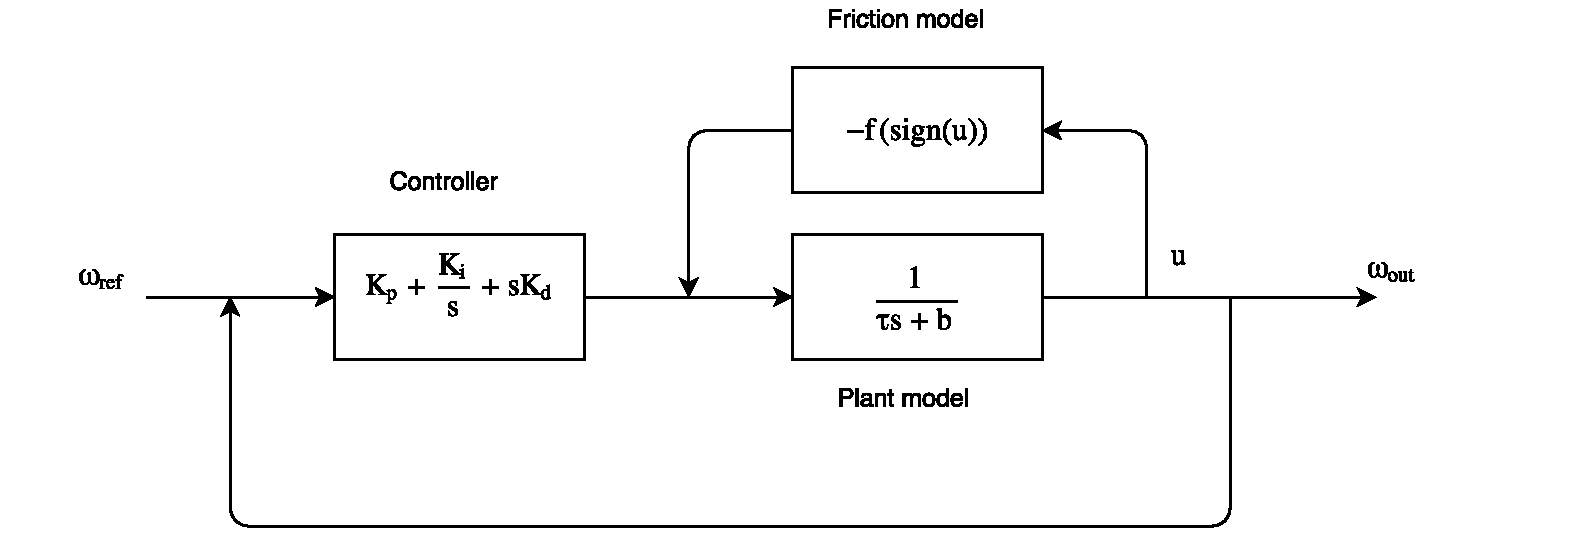
\includegraphics[width=5.5in]{res/380ModelForWheel}
    \caption[Controller for an individual Wheel]
          {Controller for an individual Wheel.}
    \label{fig:singleWheelController}
\end{figure}

The individual speed where determined through kinematic equations related individual wheel speeds to the robot's overall speed and angular velocity. Figure \ref{fig:kinematicModel} shows the kinematic model of the robot. Specifically, r describes the radius of curvature of the path, L the length of the robot, $\omega_l, \omega_r$ describes the rotation rate of the left and right wheel respectively. $V_l, V_r$ describe the linear velocities of each of the wheels. R is the radius of the wheels and $\theta$ describes the rotation about the origin. 

\begin{figure}
    \centering
    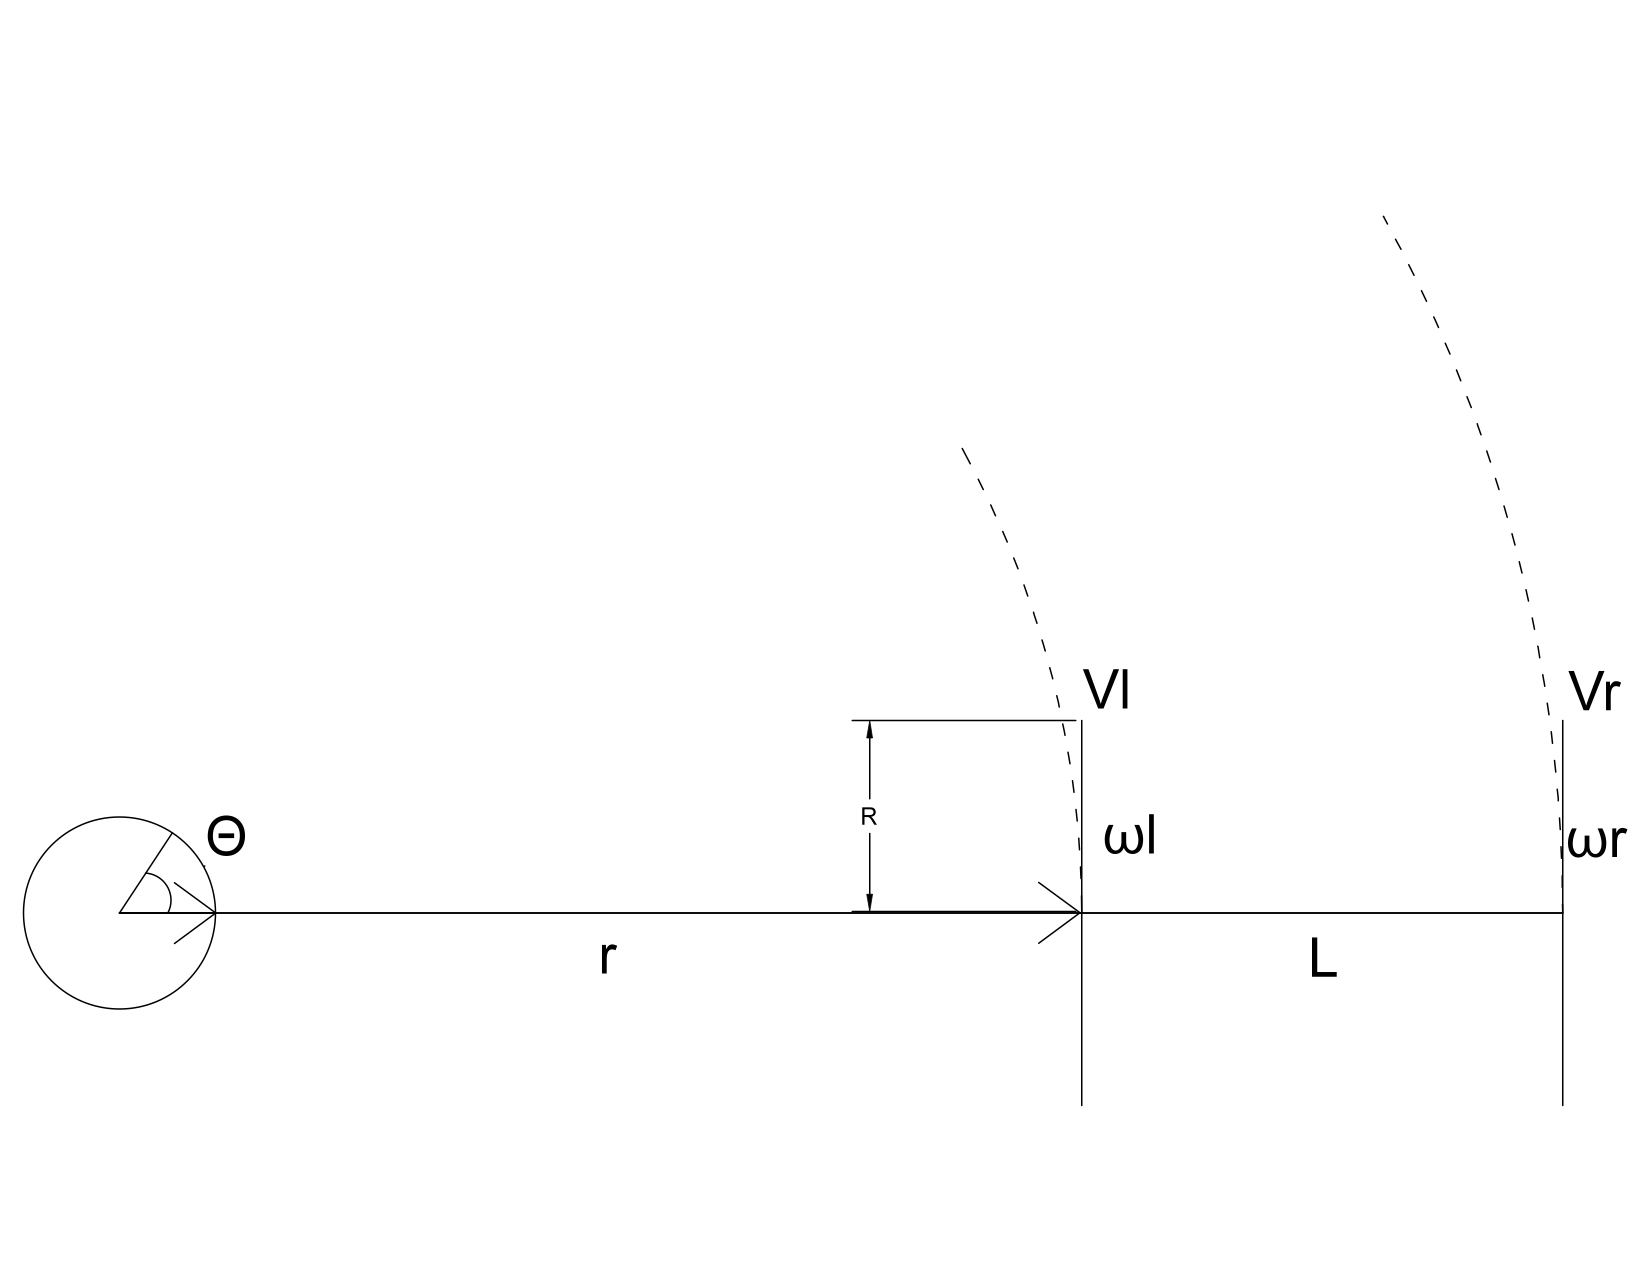
\includegraphics[width=5.5in]{res/diagram}
    \caption[Kinematic model of the robot]
          {Kinematic model of the robot.}
    \label{fig:kinematicModel}
\end{figure}

With this model the following equations can be derived, full details are found in the previous report. V and $\omega$ describe the global tangential and rotational velocities desired. It is important to note the assumptions that were made obtain these results. Mainly, that no slip exists between the wheels and the ground, and that all components within the drive train are always in contact.

\[\omega_l = \frac{2V-\omega L}{2R},\omega_r = \frac{2V+\omega L}{2R}\]
\[V=\frac{R}{2}(\omega_l+\omega_r),  \omega=\frac{R}{L}(\omega_r-\omega_l)\]

It was assumed if the wheels were individually capable of maintaining speed the robot overall would be able to follow a straight track accurately. However, this left the issue that the true variable that was desired to be controller was open loop, and error from either motor in terms of speed would result in the integration of error. The process that was used to overcome this issue is described below.

\subsubsection{Design Exploration}

During initial testing it was found to be difficult to achieve straight line driving on the platform. Through analysis of the individual wheel's speed over time, it was determined that while on average the individual speed's were very similar, bias' existed due to disturbances from construction. There are multiple root causes of this, being differing alignment on bevel gears, imperfect shafts, as well as differing motor characteristics. Overall, this caused significant turning while driving in a straight line.

A key observation made is as to now, the yaw of the robot, is being controlled in open loop. The obvious solution to this is to implement another controller around the yaw of the robot. Firstly, the following equation was derived through integration with a zero initial condition assumption.

\[\theta_r = \int\omega_rdt\]
\[\theta_l = \int\omega_ldt\]
\[\theta=\frac{R}{L}(\theta_r-\theta_l)\]

Given that there is a measure of the current angle, a PID controller can be defined to ensure that the desired angle is being outputted. The block diagram of the model is described in Figure \ref{fig:yawController}.

\begin{figure}
    \centering
    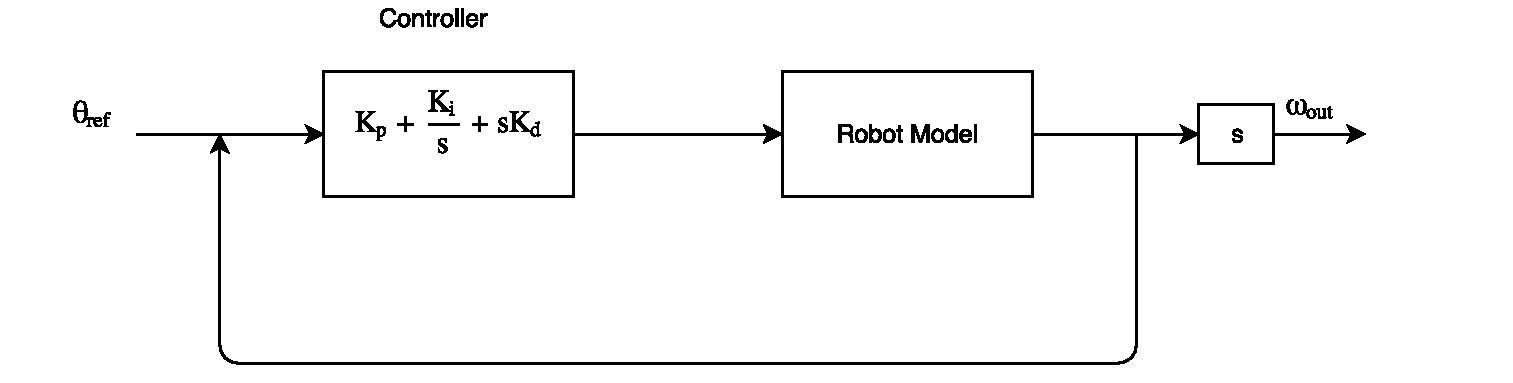
\includegraphics[width=5.5in]{res/yawController}
    \caption[Robot yaw controller]
          {Robot yaw controller.}
    \label{fig:yawController}
\end{figure}

Given the correction rotation rate as the output of the controller, corrections to the yaw can be made by changing the desired yaw being used to calculate the individual wheel speeds. In order to maintain generality the reference angle is defined as follows where $\Delta t$ is the time step between updates. 

\[\theta_{ref} = \sum\omega \Delta t\]

This ensures that the robot would achieve an angle as if it were following the desired rate of rotation over time. It is important to note that the kinematic model decouples the tangential and rotational velocities, which allowed for minimal change to the previous implementation. 

During testing it was noted that the same tuning of the controller parameters was unable to achieve stability in both the jumping and pole searching orientations of the robot. In order to combat this a gain schedule was implemented to adaptively change the tuning based on the orientation of the robot. 

\subsubsection{Key Features}

By using the full kinematic model of the system it is possible to control both the speed as well as the angular velocity of the robot through a simple interface. Moreover, since any path can be generated using a tangential and angular velocity, the implemented design is theoretically capable of physically replicating any desired trajectory with little development effort. Given the modifications, and a full model of the system, theoretical guarantees can be made about the accuracy of the position of the robot at any time. However, it is important that all times the assumptions of the system must remain valid otherwise significant tracking error will occur as described later.

\subsubsection{Testing}

During end to end testing of the robot the assumptions that were made in order to formulate the controller were strained. One of the first issues that was noticed was that after impact from landing, there was a possibility that the bevel gears within the robot were decoupled from their shafts. That is, the torque being transferred from the motor was not reaching the wheels themselves. However, presented itself as one wheel spinning slower than the other, which resulted in confusion, and doubt in the controller implementation. Moreover when the orientation of the robot in the jumping state, there were instances where the wheel did not touch the ground resulting in the robot spinning in place. These issues show the sensitivity of the algorithm to the initial assumptions that were made. Without moving the encoders to measure the output shaft or purchasing an accurate IMU to measure the overall yaw, these issues cannot be solved in software. 

Another result that was found from testing, is that when immediately commanding the motors to drive at a high speed, there was a high transient error that would not be corrected for in the length of the course ($<2$ (m)). However, this error did not exist at low speed. This lead to the conclusion that a velocity profile would act as the simplest solution to prevent any error from existing. While this was the implemented solution, it is important to note that the yaw controller itself was tuned for somewhat slower response to minimize oscillation. By increasing the performance of the controller it would be possible to achieve a better overall response with a much faster ramp up time. 

A final experiment indicated that the overall system was capable of positioning the robot better than 1 (cm) accuracy in terms of distance. Along with the high rotational accuracy, this meant that the half of the course before jumping over the wall was largely a function of human placement. Barring an orientation algorithm against the wall before jumping, localization within the course was not feasible and therefore not pursued. This prevented perfect pose within the course at all times which presented itself during the competition when the above assumptions were violated. 

Another key victory of the design was that the robot was capable of achieving the above results with significantly damaged wheel shafts. The ends of the wheels had large horizontal displacement which would have presented as large disturbances to the controller. It is likely that because the selected tuning for the controllers were not aggressive the system was less sensitive to these disturbances and was able to remain stable and accurate.
\subsubsection{Lessons Learned}

One of the key lessons learned from the implementation described is to ensure that the overall design is less susceptible to measurement errors. In this case, by either using an IMU to measure the pose, or by having the measurement done on the output, the described controller could have prevented many of the issues that took several hours of debugging. Alternatively, by implementing localization code on the robot it would have been possible to achieve the same result without having to change the robot physically. However, this is prohibitive given the limitations of the Arduino mega. 

In terms of control, a key take-away is that different orientation can cause significant dynamic changes to the system. and that significantly differing gains are required for stability. 

Lastly, while the describe system achieves high accuracy and robustness a large amount of time was devoted to tuning the controllers to achieve these results. That is, a better method of tuning, perhaps by using the serial to set the tuning values would be beneficial. 
% 
% Fan
\subsection{Pole Location Algorithm}
\subsubsection{Key Features}
\subsubsection{Design Exploration}
\subsubsection{Testing}
\subsubsection{Predicted Results Vs. Actual}
\subsubsection{Lessons Learned}
% 
% Rae
\section{Competition Result Analysis}
% 
% Daniel
\section{Conclusions}

\section{Forth Year Design Project Proposal}

%%%%%%%%%%%%%%%%%%%%%%%%%%%%%%%%%%%%%%%%%%%%%%%%%%%%%%%%%%%%%%%%%%%%%
%% BACK MATTER
%%%%%%%%%%%%%%%%%%%%%%%%%%%%%%%%%%%%%%%%%%%%%%%%%%%%%%%%%%%%%%%%%%%%%
\begingroup
\raggedright
\sloppy
\bibliography{uw-wkrpt-bib}
\endgroup

%%%%%%%%%%%%%%%%%%%%%%%%%%%%%%%%%%%%%%%%%%%%%%%%%%%%%%%%%%%%%%%%%%%%%
%% APPENDICES
%%%%%%%%%%%%%%%%%%%%%%%%%%%%%%%%%%%%%%%%%%%%%%%%%%%%%%%%%%%%%%%%%%%%%
\appendix

\end{document}